\documentclass[12pt]{article}

\usepackage{graphics}
\usepackage{graphicx}
\usepackage{amsmath} 
\usepackage{blindtext}
\usepackage{float}

\begin{document}
\title
{{\textbf{Assignment No. 1\\ }}
Minimum Distance to Class Mean classifier\\
MD. Saimom Islam\\
16.02.04.011
}

\maketitle







\section{Abstract}
\textbf{"Minimum Distance to Class Mean Classifier"} is used to classify unclassified sample vectors clustered in more than one classes are given.Basically The minimum distance classifier is used to classify unknown  data to classes which minimize the distance between the image data and the class in multi-feature space. The distance is defined as an index of similarity so that the minimum distance is identical to the maximum similarity.For example, in a dataset containing n sample vectors of dimension d some given sample vectors are already clustered into classes and some are not.we can classify the unclassified sample vectors with Class Mean Classifier.

\section {Given Task}
Given the following two class set of prototypes.Let in train.txt which level is 1 = w1 and which level is 2 = w2\\
w1 = \{(2 2 ),(3 1 ),(3 3 ),(-1 -3 )(4 2 ),(-2 -2 ) \}\\
w2 = \{(-4 3 ),(2 6 ),(0 0 ),(-4 2 ),(-1 -1 ),(-4 2 )\}\\

\subsection *{1.}
 plot all sample points from both classes,but samples from the same class  should have the same color and marker.\\
\subsection *{2.}
Using a minimum distance classifier with respect to 'class mean' , classify the following points by plotting them with the designated class-color but different marker\\
X1 = (-1 -5)\\
X2 = (3 2)\\
X3 = (-2 1)\\
X4 = (8 2)\\
X5 = (6 -1)\\
X6 = (0 2)\\
X7 = (-3 0)\\
The Linear Discriminant Function is :\\
\begin{equation*}
 g_i(X) = X^T\cdot {}_i\bar{Y}- \frac{1}{2} {}_i  \bar{Y}^T\cdot_{}i\bar{Y}
\end{equation*}

\subsection *{3.}
Draw the decision boundary between two  classes.\\
The Formula is generated from below:

Let mean1 = y1 and mean2 = y2\\\\
y1 = [1.5 .5]\\
y2 = [-1.5 2]\\

$g_1(X) = \begin{bmatrix}
1.5 & .5
\end{bmatrix}
 \begin{bmatrix}
X_1\\X_2
\end{bmatrix}\\\\
=>1.5X_1 + .5X_2 -1.25\\\\$

$g_2(X) = \begin{bmatrix}
-1.5 & 2
\end{bmatrix}
 \begin{bmatrix}
X_1\\X_2
\end{bmatrix}\\\\
=>3X_1 -1.5X_2 -1.25\\\\$

Now,For decision boundary,$ g_1 = g_2$\\

$So, \\1.5X_1 + .5X_2 -1.25 =  3X_1 -1.5X_2 -1.25\\\\
X_2 = (3X_1 + 1.878)/1.5\\$
This is the decision boundary line equation
\newpage

\section{Implementation}
1.First of all i have to plot all the sample points of both classes from train dataset.For that train data was classified in two classes based on their label.All data which are labelled 1 in one class and lebelled 2 are in another class.then the classified data are stored in two different numpy arrays,and finally plotted  with same color and marker of same class data.\\\\
2.At second step Mean of the two classes were calculated and plotted with different marker.test data were also classified based on their label and plotted with same marker and different color\\\\
3.After that the equation of decision boudary was calculated which is shown avobe and plotted every point and a decision boundary is plotted.\\\\
4.Finally the accuracy of test data was calculated compared with real class data.Using $\frac{N}{T}x100\%\ $ \\
Here N = How many samples are correctly classified and T = Total Number of samples

\newpage



\section{Main Code}
The Code is given below:



\begin{figure}[H]
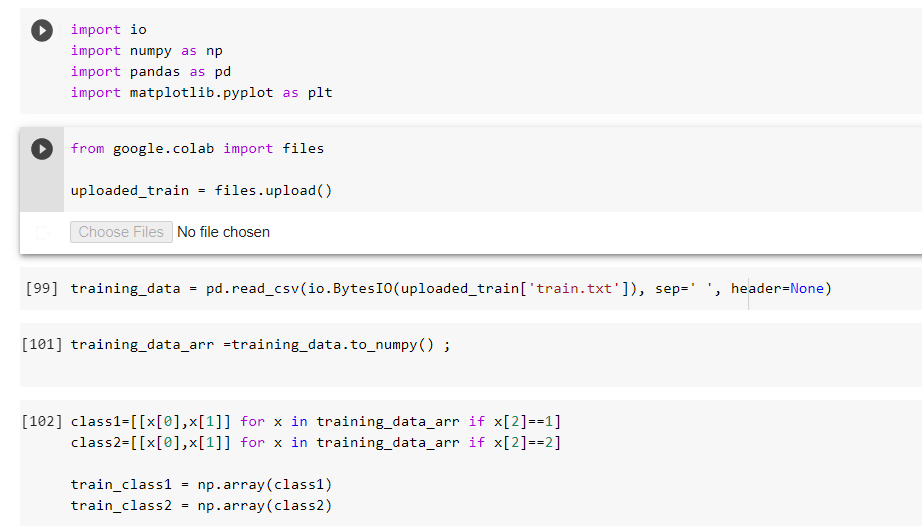
\includegraphics[scale = .7]{p1.PNG}
\end{figure}

\begin{figure}[H]
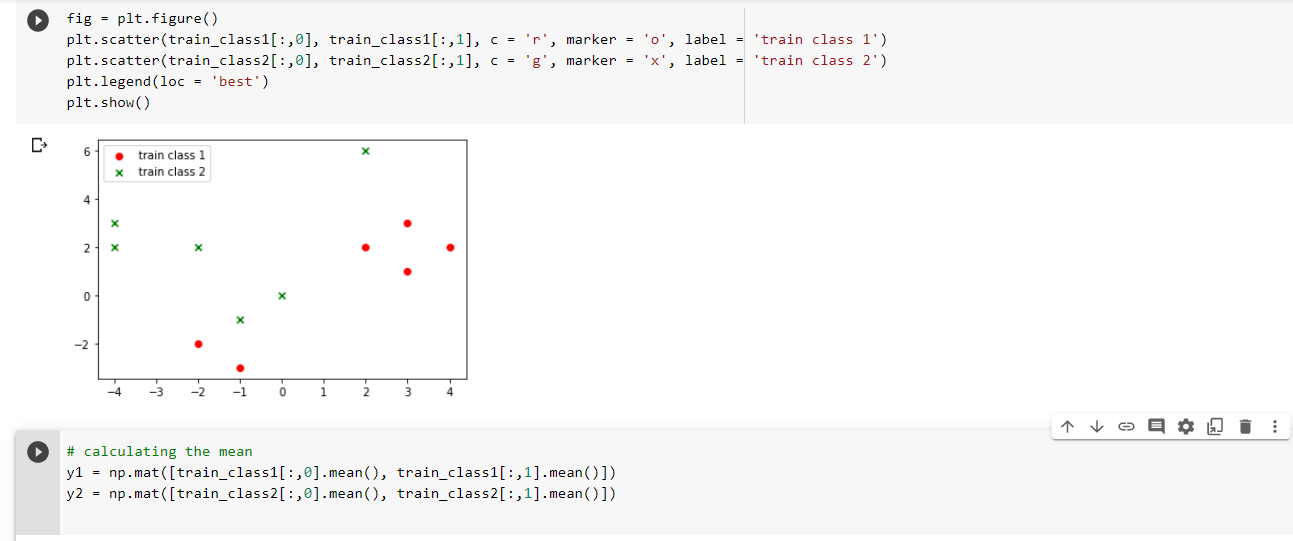
\includegraphics[scale = .7]{p2.PNG}
\end{figure}

\begin {figure}[H]
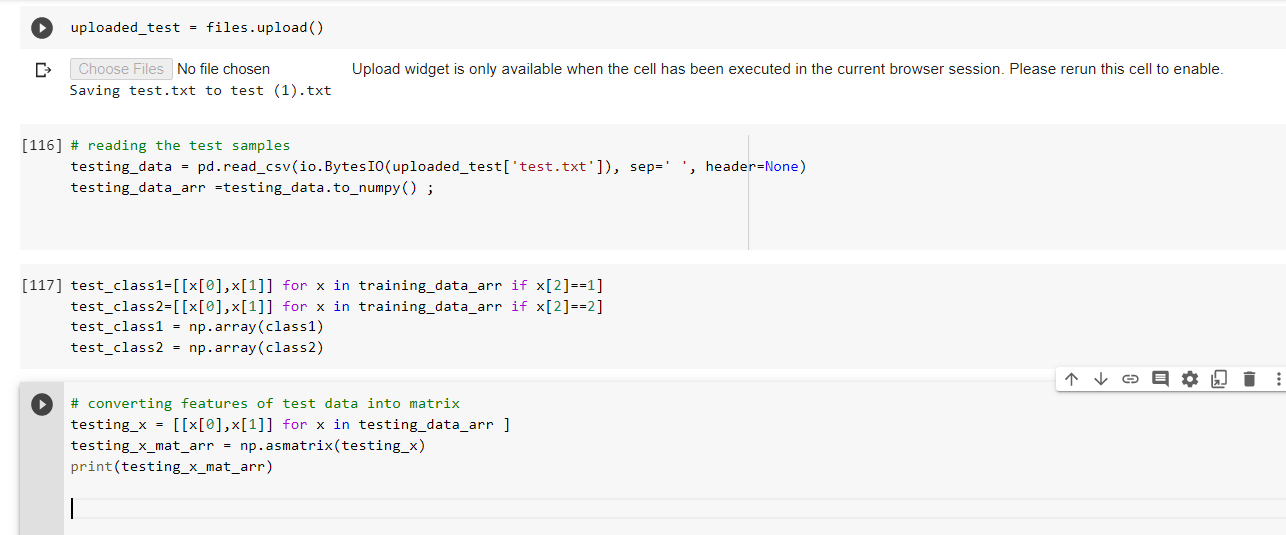
\includegraphics[scale = .7]{p3.PNG}
\end{figure}

\begin{figure}[H]
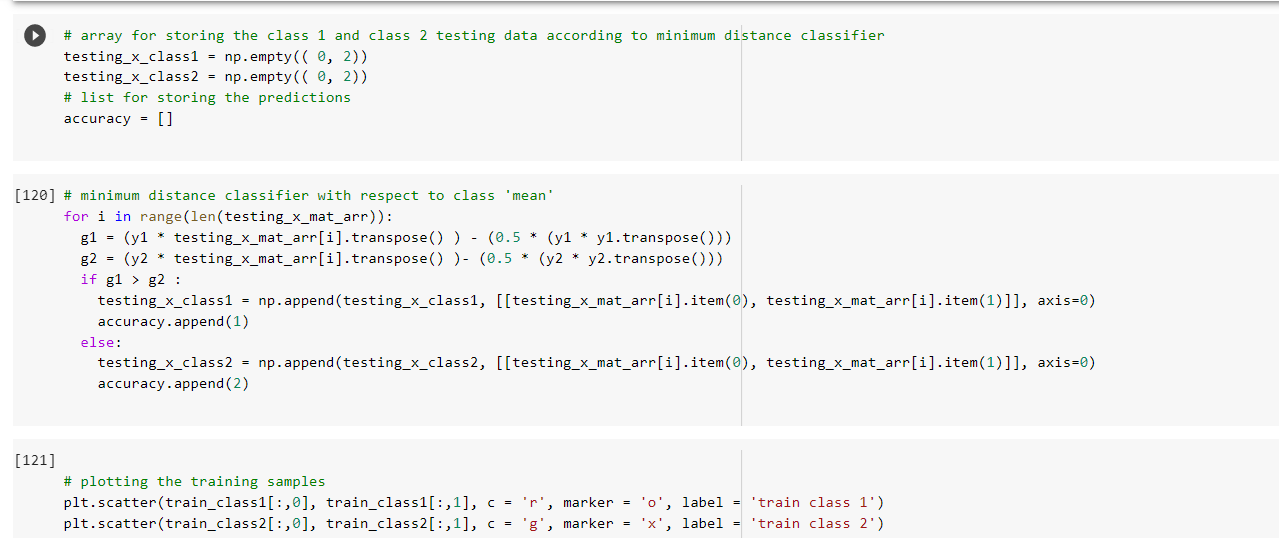
\includegraphics[scale = .7]{p4.PNG}
\end{figure}

\begin{figure}[H]
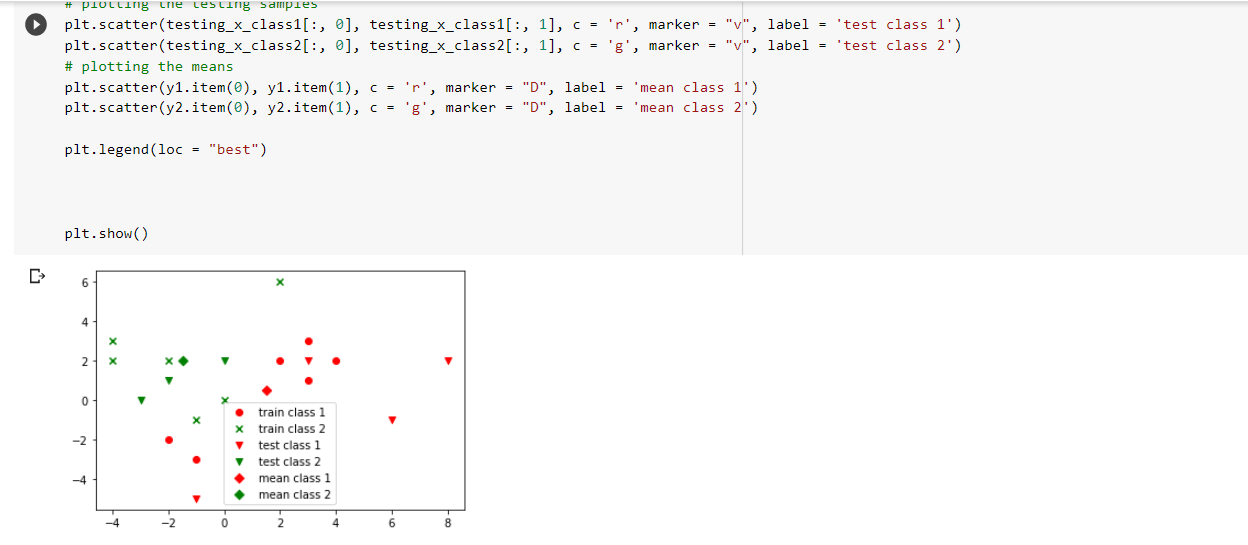
\includegraphics[scale = .7]{p5.PNG}
\end{figure}

\begin{figure}[H]
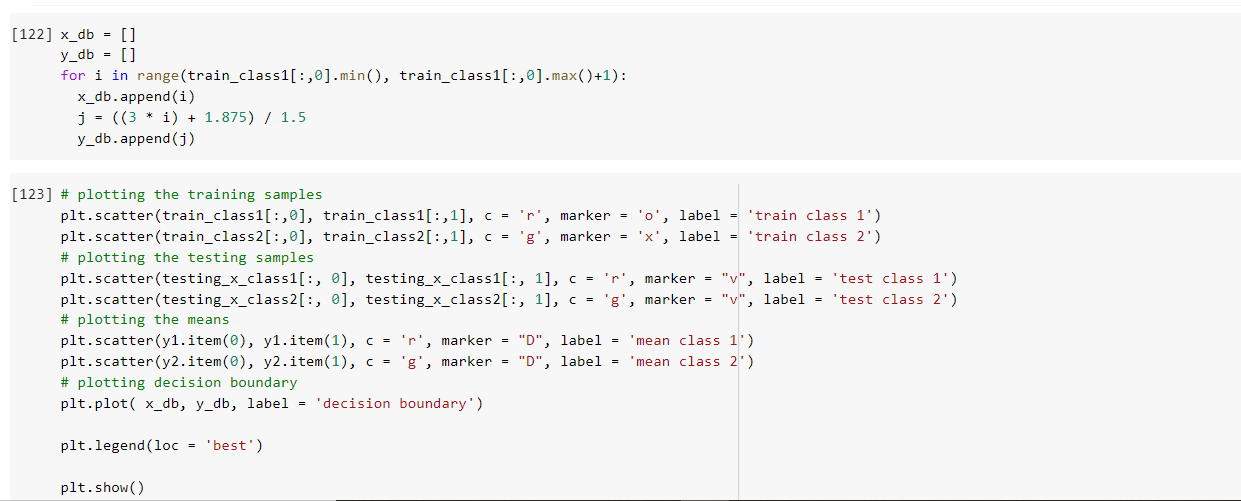
\includegraphics[scale = .7]{p6.PNG}
\end{figure}

\begin{figure}[H]
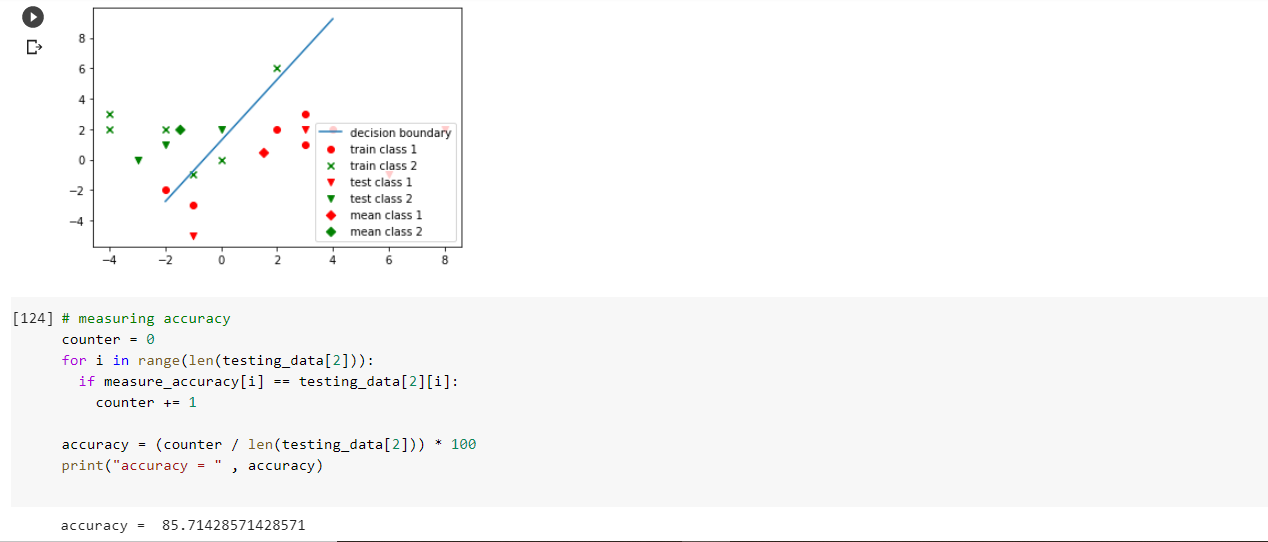
\includegraphics[scale = .7]{p7.PNG}
\end{figure}

\newpage
\section{Result Analysis}
The Results of Given tasks are given below:\\
\Large1.Plotting all sample points from training data \\


\begin{figure}[htbp]
{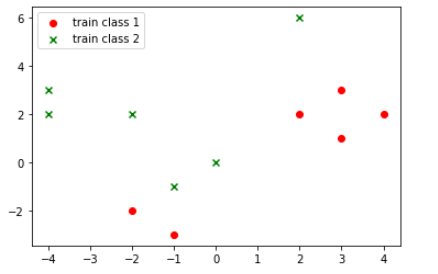
\includegraphics{res1.PNG}}
\caption{the two classes of train dataset are plotted using different marker and different color\\}
\label{fig}
\end{figure}
\newpage

2.Plotting the mean class data and test class data\\

\begin{figure}[htbp]
{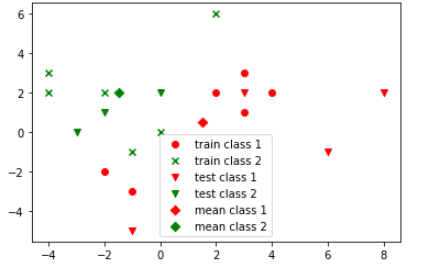
\includegraphics{2.PNG}}
\caption{Minimum distance classifier with respect to class mean and classify some sample\\}
\label{fig}
\end{figure}

\newpage

3.Plotting the decision boundary\\

\begin{figure}[htbp]
{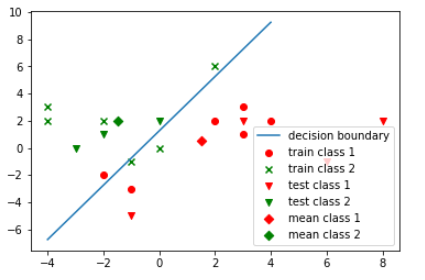
\includegraphics{3.PNG}}
\caption{Decision Boundary to classify two class\\}
\label{fig}
\end{figure}

4.Measure Accuracy\\

\begin{figure}[htbp]
{
\includegraphics{4.PNG}}
\caption{Accuracy\\}
\label{fig}
\end{figure}

\newpage





\section{Conclusion}
Minimum distance to class mean classifier is fast but the problem is it's performance is poor for big dataset.The rate of misclassification is high.Though the accuracy for this given dtaset is pretty good.the accuracy is 85.712\%.So,this classifier performed well for this given dataset


\end{document}